\documentclass{article}
\usepackage[utf8]{inputenc}
\usepackage{ragged2e}
\usepackage{parskip}
\usepackage[T1]{fontenc}
\usepackage[utf8]{inputenc}
\usepackage[table]{xcolor}
\usepackage{graphicx}
\usepackage{mathtools}
\usepackage{glossaries}
\usepackage{float}
\usepackage{pgfplots}
\usepackage{multicol}
\usepackage{subcaption}
\usepackage{pdfpages}
\usepackage[margin=3cm]{geometry}
\usepackage{listings}
\usepackage{csvsimple}
\usepackage{rotating}
\usepackage[english]{babel}

\lstset{
  basicstyle=\footnotesize,
  breakatwhitespace=false,
  breaklines=true,
  extendedchars=true,
  frame=single,
  keepspaces=true,
  numbers=left,
  showstringspaces=true,
  tabsize=4,
  title=\lstname
}

\begin{document}
  \centering        
    \vfill
    
       {\LARGE \textbf{Travaux Pratiques : Alignement local et blast}} \\[1in]
    
    \justifying
    \section{Alignement local : Smith et Waterman }
	\renewcommand{\thepage}{\arabic{page}}
	\setcounter{page}{1}
    \subsection{Principe}
Avec l'alignement des séquences locales, vous n'êtes pas contraint d'aligner l'ensemble des deux séquences comme vous l'avez réalisé avec l'alignement global; vous pouvez simplement utiliser des parties de chacune des séquences pour obtenir un score maximum. Ainsi si on utilise deux séquences S1 et S2 et la même grille de notation que vous avez vu la semaine dernière, vous obtenez l'alignement local optimal S1'' et S2'' suivant:

\begin{center}
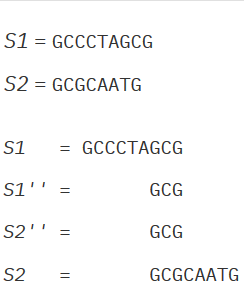
\includegraphics[width=0.2\textwidth]{figures/Aling_SW.png}
\end{center}
S1 = GCCCTAGCG\\
S2 = GCGCAATG

Dans l'algorithme Smith-Waterman, votre alignement local n'a pas besoin de se terminer à la fin de l'une ou de l'autre séquence, donc vous n'avez pas besoin de commencer votre traceback dans le coin inférieur droit; on le démarre dans la cellule avec le score le plus élevé.
\medbreak

L'algorithme Smith-Waterman diffère de l'algorithme Needleman-Wunsch en trois points :
\begin{itemize}
\item Dans l'étape d'initialisation, la première ligne et la première colonne sont toutes remplies de zéros. 
\item Deuxièmement, lorsque vous remplissez le tableau, si un score devient négatif, vous mettez 0 à la place, et vous ajoutez le pointeur en arrière seulement pour les cellules qui ont des scores positifs.
\item Enfin, dans le traçage (traceback), vous commencez par la cellule qui a le score le plus élevé et retournez à la case précédente jusqu' à ce que vous atteigniez une cellule avec un score de 0. Sinon, le traçage fonctionne exactement comme dans l'algorithme Needleman-Wunsch.
\end{itemize}	
\newpage
Voici un exemple de table résumant les différents points (match : 1, mismatch : -1, déletion : -2):

\begin{center}
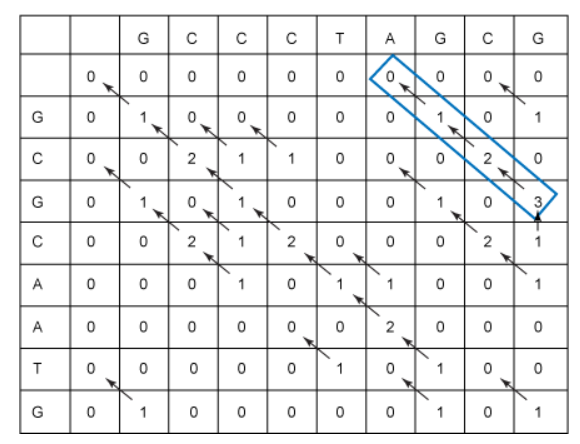
\includegraphics[width=0.5\textwidth]{figures/SWTab.png}
\end{center}

\textbf{Exercice 1 :}
Réutilisez et inspirez-vous des fonctions codées la semaine dernière pour :
\begin{itemize}
\item Construire la matrice.
\item L'initialiser.
\item Coder une nouvelle fonction qui va remplir les cellules.
\item Coder une nouvelle fonction traceback.
\end{itemize}

\newpage
	\section{Limitations}
    \subsection{Mettons notre code à l'épreuve}
    
Vous avez pu remarquer que pour un alignement quelqu'il soit, on crée une matrice de taille (taille de séquence 1*taille de séquence 2) est créée.

Alignez localement les séquences contenues dans les fichiers \textit{gene1.txt} et \textit{gene2.txt}.


    \textbf{Question :} Qu'observez vous ?
    
	\subsection{Les alignements protéiques}
	
L'alignement des séquences protéiques est plus complexe que les séquences nucléiques. Il existe 22 acides aminés chez l'Homme, on ne travaille donc plus sur un dictionnaire à 4 lettres mais à 22. Certains de ses acides aminés ont des propriétés physico-chimiques proches (voir \textit{figure 1}). 


\begin{figure}[H]
  \centering
      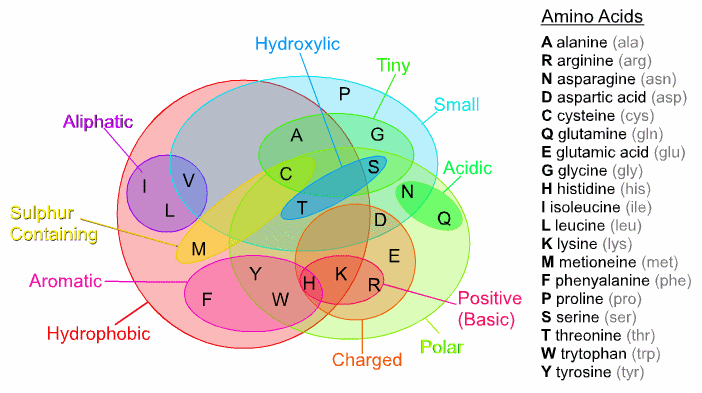
\includegraphics[width=0.8\textwidth]{figures/venn-diagram.png}
  \caption{Diagramme de Venn des propriété phisico-chimiques}
\end{figure}


Or la substitution d'un acide aminé par un autre ayant les mêmes propriétés a moins de chance d'induire un grand changement sur la fonction de la protéine. C'est pour cela qu'il a été développé des matrices de substitutions spécifiques pour tenir compte des caractéristiques des différents acides aminés. Les plus connues étant les matrices BLOSSUM (BLOcks SUbstitution Matrix) et PAM (Point Accepted Mutation).

\begin{figure}[H]
  \centering
      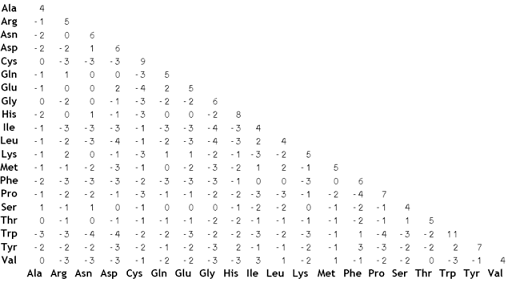
\includegraphics[width=0.8\textwidth]{figures/BLOSSUM62.png}
  \caption{Exemple de matrice de substitution BLOSSUM62}
\end{figure}

\newpage

\section{Blast : basic local alignment search tool}
\subsection{Concept}
    
Blast est un outil pour aligner localement des séquences mais il utilise une heuristique différente et plus optimisée. Cette heuristique permet notamment d'aligner une séquence face à une base de donnée qui contient une grande quantité de séquence.

Blast fonctionne en plusieurs étapes :

\begin{itemize}
\item[1] \textbf{Découpage de la séquence en k-mer :}

Le terme k-mer se réfère à tous les "sous mots"(substring) possible de longueur k contenus dans une chaîne de caractères. Par exemple, les 3-mers de la séquence ATCGATG sont ATC, TCG, CGA, GAT, ATG.

\item[2] \textbf{Énumération de tous les mots correspondants possibles :}

Tout les k-mers de taille 3 possibles (AAA,ATA,ACT...) sont alignés avec chaque k-mer de notre séquence d'intérêt. 

Les 3-mers qui ont des scores supérieurs à un seuil fixé sont gardés dans la suite des étapes.

\item[3] \textbf{Organisation des k-mers ayant obtenu le plus de points dans un arbre de recherche efficace}

\item[4] \textbf{Recherche dans la base de donnée les séquences possédant des matchs exacts avec nos k-mers retenus}

\item[5] \textbf{Extension du matchs exacts dans la séquence de la base de données :}

BLAST va alors essayer de voir si cette région homologue s'étend au-delà du k-mer de départ. Il va alors essayer d'étendre en amont et en aval du k-mer pour voir si le score d'homologie augmente avec cette tentative d'extension.

Si les deux séquences présentent effectivement une homologie locale autour du k-mer de départ, l'extension va conduire à une augmentation effective du score, car de nouveaux nucléotides vont se trouver alignés. Si au contraire la tentative d'extension ne permet pas d'augmenter le score, parce que l'homologie ne continue pas, BLAST s'arrête. Si le score final après extension est supérieur à un seuil donné, l'alignement est conservé pour l'analyse finale.

\item[6] \textbf{Analyse du score et évaluation de la pertinence :}

La recherche exhaustive avec BLAST retourne en général plusieurs dizaines d'alignements avec la séquence d'intérêt. Cependant, on ne peut rejeter l'hypothèse que ces résultats soient du au hasard (les bases de données contiennent énormément de séquences). BLAST évalue ses alignement en analysant la distribution des scores d'alignement entre la séquence d'intérêt et la banque. Il ajuste cette distribution à une fonction de densité théorique, ce qui lui permet de calculer la probabilité et l'espérance mathématique de trouver un alignement donnant un score donné dans la banque, uniquement du fait du hasard. Les paramètres de cette fonction de densité varient en fonction des compositions en nucléotides ou acides aminés de la séquence et de la banque analysée.
\end{itemize}

\subsection{Les différents Blast}

Différents outils blast existent et sont optimisés pour certains types de données ou pour réaliser des alignemnents particuliers.

\begin{itemize}
\item \textbf{blastn} : alignement de nucléotides, séquence nucléotidique contre une base de données de séquences nucléotidiques.

\item \textbf{blastp} : alignement de protéines, séquence de protéine contre une base de données de séquences de protéines.

\item \textbf{blastx} : alignement de séquence nucléotidique traduite en séquence de protéine contre une base de données de séquences de protéines.

\item \textbf{tblastn} : alignement de séquence de protéine contre une base de données de séquences nucléotidiques traduites en séquences de protéines

\item \textbf{tblastx} : alignement de séquence nucléotidique traduite en séquence de protéine contre une base de données de séquences nucléotidiques traduites en séquences de protéines.
\end{itemize}

\subsection{Utilisation de Blast en ligne}

Nous allons maintenant utiliser Blast en ligne et voir les possibilités qu'il y a derrière en terme d'anlyse.

\begin{itemize}
\item Allez sur https://blast.ncbi.nlm.nih.gov/Blast.cgi, et choisissez blastn

\item Chargez le fichier sequence-unknown.txt dans "Enter Query Sequence".

\item Dans "Program selection", choisissez blastn.

\item Activez l'option "Show results in a new window".

\item Lancez le BLAST.

\item Quel résultat obtenez vous ? A quoi semble correspondre la séquence ?

\item A quoi correspond le max score,total score, la query cover, l'e-value et l'identité ? (Aidez-vous de l'aide en ligne de blast)

\item Retournez sur la page indiquée précédemment et cliquez sur blastx.

\item Lancez une requête avec la \textit{sequence-unknown.txt}.

\item Quelles informations supplémentaires avez vous accès ?

\item Combien de domaines d'activités sont référencés ? Dans quelle région ?
\end{itemize}

\textbf{Bonus :} Il est possible de modifier plusieurs paramètres dans les différents outils de BLAST (dans Algorithm parameters). Modifiez-les et observez s'il y a des différences.
  \end{document}
